% This must be in the first 5 lines to tell arXiv to use pdfLaTeX, which is strongly recommended.
\pdfoutput=1
% In particular, the hyperref package requires pdfLaTeX in order to break URLs across lines.

\documentclass[11pt]{article}

% Remove the "review" option to generate the final version.
\usepackage{ACL2023}

% Standard package includes
\usepackage{times}
\usepackage{latexsym}

% For proper rendering and hyphenation of words containing Latin characters (including in bib files)
\usepackage[T1]{fontenc}
% For Vietnamese characters
% \usepackage[T5]{fontenc}
% See https://www.latex-project.org/help/documentation/encguide.pdf for other character sets

% This assumes your files are encoded as UTF8
\usepackage[utf8]{inputenc}

% This is not strictly necessary, and may be commented out.
% However, it will improve the layout of the manuscript,
% and will typically save some space.
\usepackage{microtype}

% This is also not strictly necessary, and may be commented out.
% However, it will improve the aesthetics of text in
% the typewriter font.
\usepackage{inconsolata}

\usepackage{amsmath,amssymb,amsfonts}
%\usepackage{ebgaramond-maths}
\usepackage{algorithmic}
\usepackage{graphicx, subcaption}
\usepackage{textcomp}
\usepackage{xcolor}
\usepackage{float}

% If the title and author information does not fit in the area allocated, uncomment the following
%
%\setlength\titlebox{<dim>}
%
% and set <dim> to something 5cm or larger.

\title{Detecting Deception in Enron Emails}

% Author information can be set in various styles:
% For several authors from the same institution:
% \author{Author 1 \and ... \and Author n \\
%         Address line \\ ... \\ Address line}
% if the names do not fit well on one line use
%         Author 1 \\ {\bf Author 2} \\ ... \\ {\bf Author n} \\
% For authors from different institutions:
% \author{Author 1 \\ Address line \\  ... \\ Address line
%         \And  ... \And
%         Author n \\ Address line \\ ... \\ Address line}
% To start a seperate ``row'' of authors use \AND, as in
% \author{Author 1 \\ Address line \\  ... \\ Address line
%         \AND
%         Author 2 \\ Address line \\ ... \\ Address line \And
%         Author 3 \\ Address line \\ ... \\ Address line}

\author{David Hobson \and Caleb Moses \and Svetla Vassileva \\
  \texttt{\{david.hobson, caleb.moses, svetla.vassileva\}@mail.mcgill.ca} \\
  \textit{dept. of Computer Science, McGill University, Montreal, Canada}}


\begin{document}
\pagestyle{plain}
\thispagestyle{plain}

\maketitle
\begin{abstract}
In this paper we explore the possibility of identifying a fraudulent actor based on their language. We consider the email dataset of Enron employees which includes emails from convicted offenders and regular employees. We look at fraud through the prism of deception, verifying if known markers of deception correlate with fraud. We also look for new potential language markers that could correlate to fraud. The code is available on GitHub\footnote{\url{https://github.com/mathematiguy/enron-nlp-analysis}}.
\end{abstract}

%To this end,
% ranging from convicted offenders to regular employees

\section{Introduction}
Identifying deception is a difficult task \cite{mafia}. While humans usually act collaboratively, people can be incentivized to lie or deceive others for many reasons. %, whether to avoid confrontation or conflict, to avoid losing face, or for nefarious reasons including personal gain or the achievement of some criminal objective. 
Previous studies have shown that people can struggle with identifying lies from truths \cite{mafia}. Even trained law enforcement professionals are only slightly better than chance at detecting deception \cite{enron_deception_gupta}.

Many works have studied and identified different computational linguistic features which are correlated with deceptive actions in controlled environments, for example in games like \textit{Diplomacy} \cite{diplomacy} and \textit{Mafia} \cite{mafia}. In this work we speculate as to whether such deceptive patterns apply to more complex real-world settings, such as fraud detection.

Among the most famous fraud cases is the collapse of Enron, the American energy company that filed for bankruptcy in 2001 after widespread fraud within the company was revealed by the media. In the aftermath of the scandal, several Enron executives and employees were convicted or pleaded guilty of fraud and related crimes.

Since the collapse, some of the emails from Enron employees discovered in the course of the court case have been made public. This dataset includes emails leading up to the events and in particular from high-profile executives who were ultimately convicted \cite{enron_dataset}. This Enron email dataset is a unique testbed for the study of markers of fraud and deception in a real-world scenario.

Combining this with the prior research studying deception in games, the goal of this project was to analyze the Enron email dataset, and observe whether the same markers of deception that are displayed in game environments are also present within the emails of Enron employees who were eventually convicted of fraud.

We further train our own classifiers to identify emails written by fraudsters, and assess the linguistic features it finds most useful. 

%\textbf{What is the hypothesis that you test and how do you go about doing so?}
%
%To this end, we... 
%
%It turns out that...
%
% This project provided an exciting opportunity to dive into this ``true crime'' world and investigate the nature of fraud from a language analysis prospective. Fraud presupposes deception and we therefore leaned into identifying deception from text. 

% We then proceed to search for other potential markers. The only one that stood out was negative sentiment. We explore the correlation between negative sentiment and fraud. 


% was not statistically significant. 


% It turns out that, indeed, none of the deception markers identified in [danescu] can be applied transversally to the deception in Enron. 




\section{Related Work}
% Various works have studied linguistic cues related to deception, as well as similar phenomena like betrayal, in the context of games. 

Niculae et al. \cite{diplomacy} developed a framework for analyzing evolving dialogues in the game of \textit{Diplomacy}: a war-themed strategy game where players converse to form alliances, but must ultimately betray their allies to gain territory and win the game. In particular, they found that imminent betrayal was signaled by sudden, but slight, increases in positive sentiment and politeness on the part of the betrayer. The use of planning discourse markers was also found to correlate with betrayal, with betrayees typically using them more often than betrayers just before the deception.

% In recent work, Ibraheem et al. \cite{mafia} studied deception in the game of \textit{Mafia} where players are assigned a mafioso or a bystander role, with the objective being to either to learn the identities of all the mafiosos (for the bystanders) or to eliminate all the bystanders (for the mafiosos). Mafiosos are thus highly incentized to deceive the bystanders, whereas the bystanders are incentized to play an honest role. Ibraheem et al. applied two approaches to this problem: a standard BERT-based classifier that only used the utterances of the player to be classified, and a second auxiliary approach that also accounted for prior utterances from all players. They found that accounting for past utterances improved performance, and suggested that linguistic behaviour like referring to other players (especially for elimination), and asking for suggestions on how to eliminate were stronger indicators of mafiosos, whereas aspects of confusion may be more strongly correlated with bystanders. 

This work provides insights into the subtle cues associated with deception. However the setting of a game is highly constrained: the environment is highly simplified compared to the real world. We expect that finding signs of deception in a free-form and open world, such as in the Enron case, will be more difficult. 

% Tie this in somehow:
%The italian court cases are from 2013, the diplomacy paper from 2015, too long to explain connection and differences

Several works have analyzed the Enron dataset in the past, specifically applying different models of deception. In particular, Gupta et al. \cite{enron_deception_gupta} and Keila et al. \cite{enron_deception_keila} both characterized deception by a reduced usage of first-person pronouns and exception words, and an increased usage of negative emotions words and action verbs. They each applied SVD to the emails, and found these latent factors in deceptive emails.

In other work, Eckhaus et al. \cite{hubris} investigated the use of words specifically linked to hubris. They found that among the executives eventually convicted, their usage of hubristic terms increased in frequency prior to the collapse. In this way, they illustrated a trend possibly correlated to deception, which suggests the potential existence of predictive features that could be used in other circumstances to identify signs of deception or deterioration. 

% As fraudulent practices at Enron had been going on for years if not decades, there is no specific ``deception moment''. We focus on the brief period that precedes the bankruptcy, as language might be likely to change around this time of reckoning, and deception of shareholders and the public was at its conscious peak. %The first signs of doubt appeared in the public space in the beginning of 2001 \cite{fortune}, leading up to the bankruptcy filing at the end of the same year (on December 2nd). We take October 2001 to be the beginning of the collapse, since it is at that time that the signs were apparent to the public (Enron's stock price started decreasing sharply, never to recover(CITATIONS)) and simultaneously, internal deception was provably practiced (Enron's legal council had requested auditors to destroy documents \cite{andersen-docs}). We therefore turn our attention to the beginning of October 2001. 

Motivated by this work, we apply a similar approach but with the deception features identified by Niculae et al. As fraudulent practices at Enron had been going on for years, there was no specific ``deception moment''. However, we observe the trends of positive sentiment, politeness, and planning discourse before and during the collapse to see whether there is a difference between individuals who were and were not convicted of crimes. Our hypothesis is that these markers of deception are transferable to a different real-life context. 

To further explore the space of good predictive features for deception at Enron, we trained linear classifiers to extract tokens that are most useful to predicting a fraudster. 


\section{Method}
\subsection{Dataset}

We use the Enron Email Dataset \cite{enron2015email} provided by Dr. William W. Cohen, specifically, the May 7, 2015 version of the dataset. The dataset contains 517,401 emails from employees at Enron that were obtained by the Federal Energy Regulatory Commission during its investigation of Enron's collapse. 

As this dataset only contains emails and little metadata, information about the authors was supplemented using additional sources. A \textit{New York Times} \cite{nytimes} archive was used to identify individuals who were convicted of crimes related to the collapse. Of these individuals, only four had emails present in the dataset, namely Kenneth Lay, Jeffrey Skilling, David Delainey, and John Forney. We shall refer to these individuals as persons-of-interest (POIs) from this point forward.

\begin{table}[t]
    \centering
    \caption{The breakdown of emails in our dataset including the number of emails in the training, validation, and test sets, and the number of POI, executive, and normal employee emails in each.}
    \label{tab:dataset_breakdown}
    \resizebox{0.48\textwidth}{!}{%
    \begin{tabular}{|l||r|r|r|r|}
        \hline
         & \textbf{POI} & \textbf{Executive} & \textbf{Normal} & \textbf{Total} \\
        \hline
        \hline
        Training & 670 & 1,807 & 5,467 & \textbf{7,944} \\
        \hline
        Validation & 167 & 450 & 1,369 & \textbf{1,986} \\
        \hline
        Test & 272 & 774 & 2,264 & \textbf{3,310} \\
        \hline
        \textbf{Total} & \textbf{1,109} & \textbf{3,031} & \textbf{9,100} & \textbf{13,240} \\
        \hline
    \end{tabular}%
    }
\end{table}

As all the POIs were executives at Enron, further information was collected to identify other executives in the dataset who were not eventually convicted of fraud. This was to ensure a fair comparison, and to add confidence that any features associated with POIs were not more broadly applicable to other executives. A dataset \cite{enron_financial_dataset} of financial information, while not containing any explicit information on employees' positions, was used to identify individuals similar to executives. For the purposes of this project, anyone with a salary above $\$200,000$ USD per year was considered an executive.
%The dataset \cite{enron_financial_dataset} of financial information does not contain explicit information on employees' positions, but the salary information was used to identify individuals similar to executives. For the purposes of this project, anyone with a salary above $\$200,000$ USD per year was considered as an executive.



%A dataset of financial information was found \cite{enron_financial_dataset}, and while this dataset did not contain explicit information on employees' positions, the salary information was used to identify individuals similar to executives. 

A subset of the emails was used which consisted of emails from 22 authors: the 4 POIs (Lay, Skilling, Delainey, and Forney), 5 other executives who were not convicted of crimes, as well as 13 other ``normal" employees at Enron who were neither POIs nor executives. This uneven corporate rank distribution was chosen to reflect a more accurate employee-to-executive ratio to what might be expected in other companies. Overall, roughly 700 emails were taken from each person to ensure each author was similarly represented. This, however, was only applied to executives and normal employees, to ensure the fraction of POI emails would remain low. %This was to reflect the expectation that in a normal organization, the number of frauds would be expected to be low. 
In particular, our email subset contained 13,240 emails with 8.3\% of emails from POIs, 22.9\% of emails from execs, and 68.8\% of emails from normal employees. 

In terms of the authors chosen, the executive emails were taken from Allen, Kitchen, Lavorato, Shankman, and Shapiro. For the normal employee emails, they were taken from Bass, Dasovich, Davis, Germany, Jones, Lenhart, Mann, Nemec, Perlingiere, Rogers, Scott, Shackleton, and Symes. These authors were chosen since they had a large number of emails in the original Enron dataset.

% Further cross-referencing with an article of the \textit{Financial Times} \cite{enron_financial_dataset}, which contains the income of many Enron employees, allowed us to annotate many of the email authors according to their status in the company. We refer to the employees with incomes above \$200K as execs, sometimes also differentiating higher execs (income over \$300K). This is important to avoid social status bias in politeness classification (cite someone who says low politeness correlates with high status?????). Authors for whom we were unable to find income information were assumed to be of ``normal'' income. 

\subsection{Data Cleaning}

% One major data processing step was to annotate the emails with extra information about the authors. Cross-referencing with an article in the \textit{New York Times} \cite{nytimes} which summarizes the outcomes of the Enron trials allowed us to identify authors that were convicted of, or plead guilty to, fraud. Since the Enron data set is not a complete collection of all emails written by Enron employees over the years, there were only four authors (Lay, Delainey, Skilling, Forney) who were convicted of fraud. Throughout our work, they are referred to as POI (people of interest). Further cross-referencing with an article of the \textit{Financial Times} \cite{enron_financial_dataset}, which contains the income of many Enron employees, allowed us to annotate many of the email authors according to their status in the company. We refer to the employees with incomes above \$200K as execs, sometimes also differentiating higher execs (income over \$300K). This is important to avoid social status bias in politeness classification (cite someone who says low politeness correlates with high status?????). Authors for whom we were unable to find income information were assumed to be of ``normal'' income. 

Emails were gathered using the email addresses of the relevant individuals. Any email address that contained the name of an individual was used for that particular author.

Since our focus was on the language of the authors themselves, careful selection was done to ensure that only emails written by the actual authors were kept. Forwarded and replied text was removed, as well as messages written by the secretaries or assistants of the individuals. This was done programmatically using the names of secretaries discovered in random samples of the dataset. While it is still possible that some emails may have been written by other individuals, for the emails of the POIs all emails were manually inspected to ensure they were all written by the sender. 

Additional data cleaning involved removing empty and duplicate emails. Finally, only emails consisting of 5 words or more were kept, and all emails sent from before 1999 were also dropped since they only accounted for about 100 emails.

\subsection{Modeling}

Following Niculae et al., we model the positive sentiment, politeness, and planning discourse markers in the emails.

For sentiment, the \textit{SiEBERT} \cite{sentimentModel} model from Huggingface was used. It is a fine-tuned checkpoint of RoBERTa-large, originally evaluated on diverse datasets coming from reviews, tweets and other similar sources. 

For the politeness model, a pre-trained politeness model trained on the Wikipedia Politeness Corpus was used provided in the ConvoKit package.

To study planning discourse, we collated a list of individual (single-word) and phrasal (bi-gram) planning discourse markers. The individual markers we chose were "shall", "going", "planning", "intend", "aim", "hope" and "expect", and the phrasal markers we chose were "plan to", "aim to", "looking forward", "in preparation" and "prepare for". For each class, and each month, we totaled the number of planning discourse markers we were able to match and divided by the number of sentences in the sample, as identified by NLTK. This gave us the percentage of planning discourse markers per sentence per month across each of the 3 employee classes under consideration.

Finally, for training our own classifiers, we tested a mix of 24 different logistic regression and naïve Bayes models to predict whether an email was written by a POI. These models varied in the text preprocessing step or in the hyperparamter value (smoothing parameter for naïve Bayes, and regularization strength for logistic regression). 

While these models are only linear classifiers, they were chosen due to their interpretability since the feature weights and probability values can measure the relative importance of the different words in the predictions.

% Note that for the naïve Bayes models, the \texttt{ComplementNB} model was used in scikit-learn since this variant is better suited to imbalanced datasets, like the one here. 

\subsection{Text Preprocessing}

% All emails were cleaned, as described above, before further processing.

For the sentiment analysis, politeness, and planning discourse markers, the emails were passed as-is to the model pipelines. 

For classification, entities for organizations, locations, and people names were masked in the emails. This was done to avoid the models from learning Enron-specific features in the emails, as the goal was to find linguistic cues that were as generalizable as possible to other deception/fraud domains. Specifically, all names were replaced by ``Steve'', all organizations by ``Apple'' and all locations by ``Cupertino''.

Emails were tokenized and lemmatized using NLTK. Stopwords were removed using NLTK's list of stopwords, and standard punctuation and digits were removed. Experiments involving stemming and bigrams were completed, however these models did not perform as well as unigram models.

Words were vectorized using TF-IDF. Other vectorization schemes including embeddings and other pre-trained methods were not attempted in order to preserve the explainability of the features. 

\subsection{Evaluation}

The classifiers were trained on the training set, and hyperparameters and the choice of best model was based on the F1 score of the POI class on the validation set. The F1 score was used due to the heavily imbalanced nature of the dataset. For the training/validation/test split, see Table \ref{tab:dataset_breakdown}.

The final evaluation reported in Table \ref{tab:best_model_metrics} is based on the precision, recall, and F1 score of the POI class on the test set.


\section{Results}
%%%% Establishing the collapse period -- does not belong in results? 
% As fraudulent practices at Enron had been going on for years if not decades, there is no specific ``deception moment''. We focus on the brief period that precedes the bankruptcy, as language might be likely to change around this time of reckoning, and deception of shareholders and the public was at its conscious peak. 
% The first signs of doubt appeared in the public space in the beginning of 2001 (cite WIKIPEDIA on ENRON scandal), leading up to the bankruptcy filing at the end of the same year (on December 2nd). We take October 2001 to be the beginning of the collapse, since it is at that time that the signs were apparent to the public (Enron's stock price started decreasing sharply, never to recover, and the company's credit rating was downgraded) and simultaneously, internal deception was provably practiced (Enron's legal council had requested auditors to destroy documents). %We therefore turn our attention to the beginning of October 2001. 

% The first signs of doubt appeared in the public space in the beginning of 2001, leading up to the bankruptcy filing on December 2nd of that year. We take October 2001 to be the beginning of the collapse since this was when it went public, and simultaneously, internal deception was provably practiced (Enron's legal council had requested auditors to destroy documents). 

Figures \ref{fig:politeness}, \ref{fig:discourse} and \ref{fig:sentiment} show the politeness, planning discourse, and sentiment levels respectively  in emails of the POIs, executives, and normal employees. 

The politeness of the execs and regular employees appeared to remain more or less constant throughout. However, in the POI emails, there was a distinct increase in politeness prior to the collapse, followed by a sharp drop thereafter, confirming the results in \cite{diplomacy}. 

\begin{figure}[b!]
    \centering
    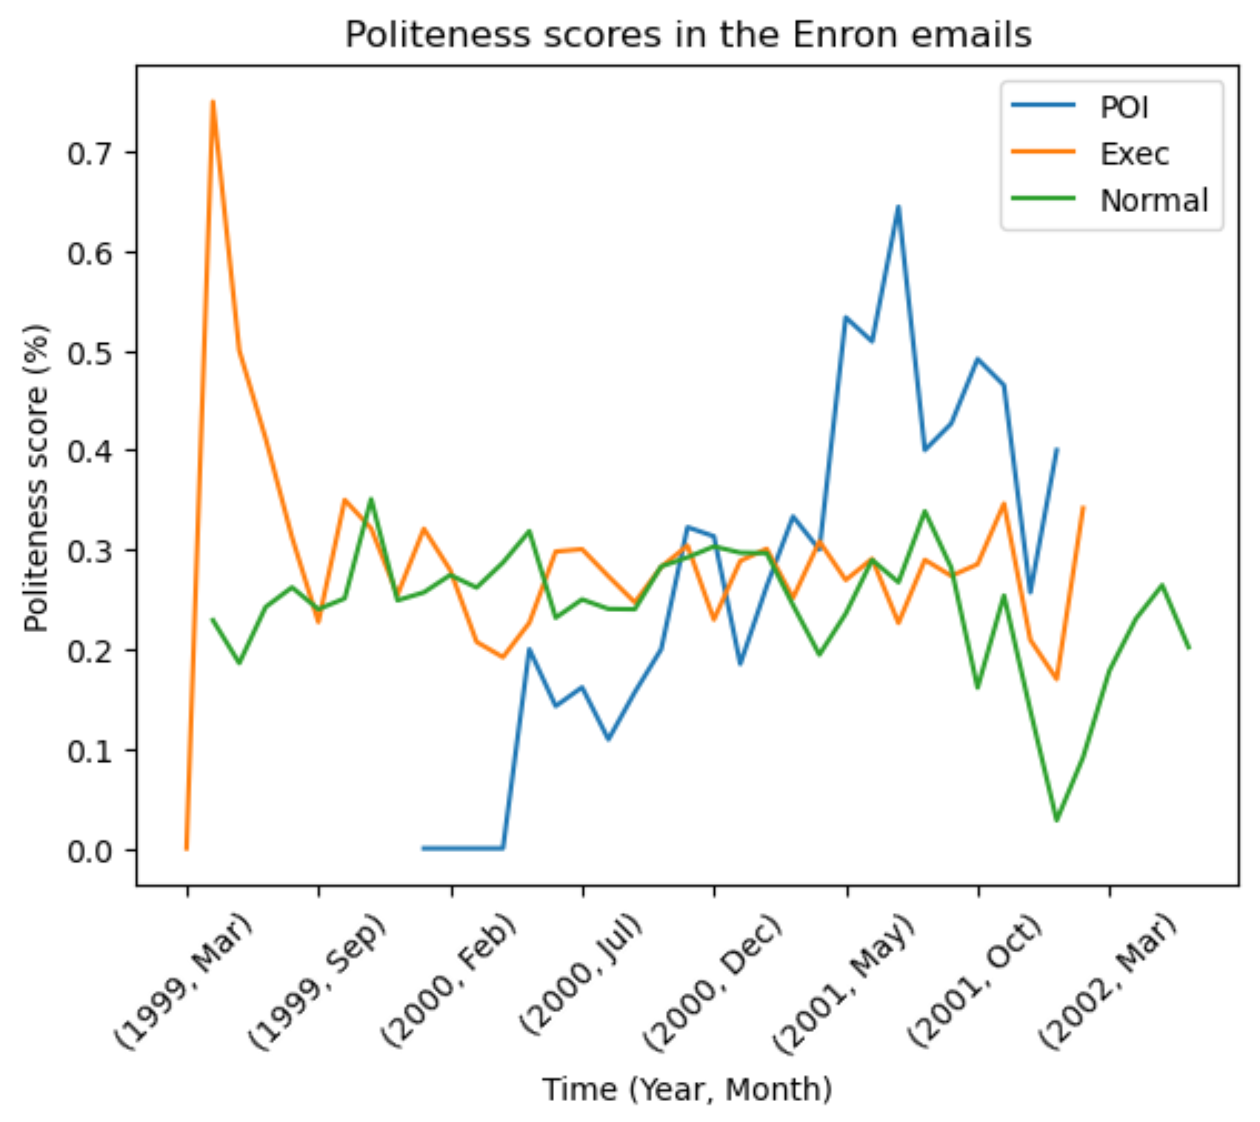
\includegraphics[width=8cm]{images/politeness_plot.png}
    \caption{Politeness scores produced by the Stanford politeness classifier}
    \label{fig:politeness}
\end{figure}

\begin{figure}[b!]
    \centering
    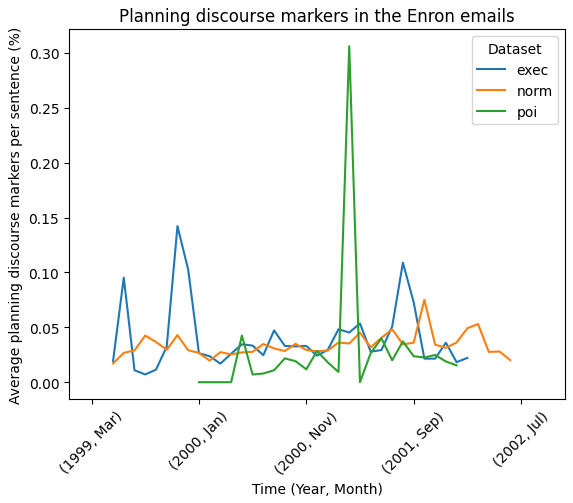
\includegraphics[width=8cm]{images/discourse_plot.png}
    \caption{Percentage of planning discourse markers per sentence in the Enron emails}
    \label{fig:discourse}
\end{figure}

The planning discourse frequencies in Figure \ref{fig:discourse} similarly showed a concordance with the features in \cite{diplomacy}. There is a clear spike in planning discourse which happens in March 2001 -- a time that coincides with the first public questioning of Enron's solvency in a \textit{Fortune} article \cite{fortune}. While it is impossible to assert a causal relationship, it should be noted that all data anomalies observed do line up with major events in the Enron collapse, and are isolated to only POI emails and not the general executive emails. %Similarly to Figure \ref{fig:politeness}, the trends for normal employees and executives appear to remain relativity stable compared to the POI results.

Figure \ref{fig:sentiment} did show a departure from the findings of \cite{diplomacy} where no clear increase in positive sentiment among the POI emails was seen. %In fact, the plot seemed to show a slight downward trend in sentiment for the POIs, a slight increase in sentiment for the normal employees, and a consistent sentiment for the other executives. 

Table \ref{tab:best_model_metrics} gives the model parameters and evaluation metrics for the best performing classifier trained. As seen, the model was competent at identifying POIs. This is promising given the presence of other executives in the data, and thus shows the models are able to identify features pertinent to POIs but not executives more broadly.

Figure \ref{fig:features} shows those features that were most useful for detecting fraudulent activity. %It is doubtful that a specific words (e.g., `ensure') would be indicators of a person's deceitful intentions, however 
Several features (`dont', `however', `doesnt') seemed to suggest a pattern of negative sentiment may be related to fraud, however it is interesting to note that this was not reflected in Figure~\ref{fig:sentiment}%, and therefore while these particular words may be related to detecting frauds, negative sentiment in general does not appear to be useful. However further work may be required to confirm this.

% \begin{figure}[t!]
%     \centering
%     \begin{subfigure}[b]{0.4\textwidth}
%         \centering
%         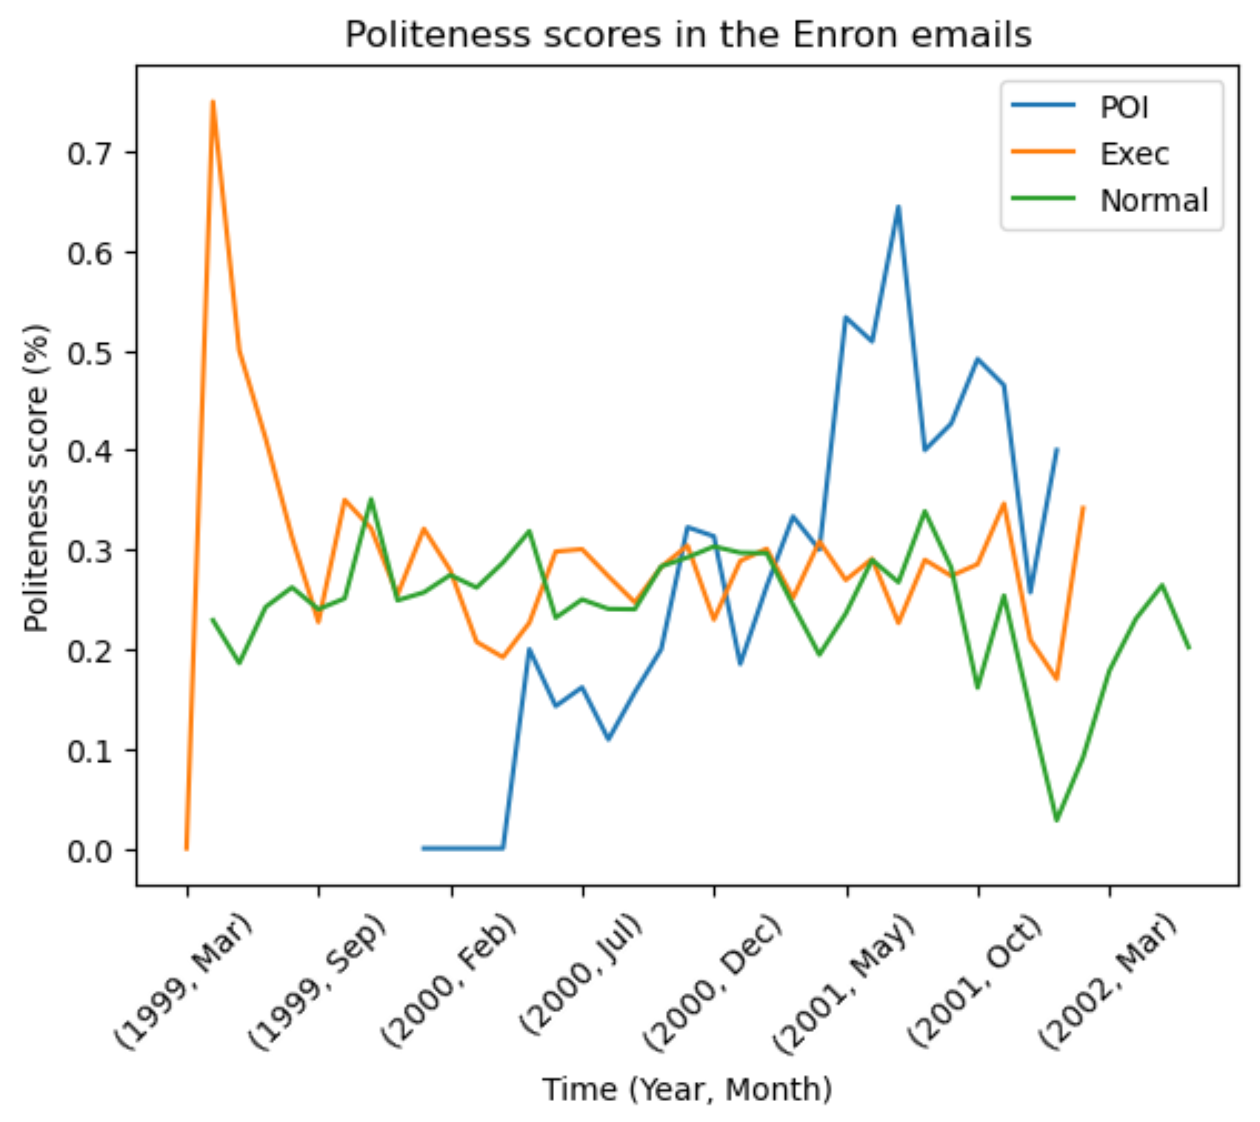
\includegraphics[width=8cm]{images/politeness_plot.png}
%         \caption{Politeness scores produced by the Stanford politeness classifier}
%         \label{fig:politeness}
%     \end{subfigure}
%     \begin{subfigure}[b]{0.4\textwidth}
%         \centering
%         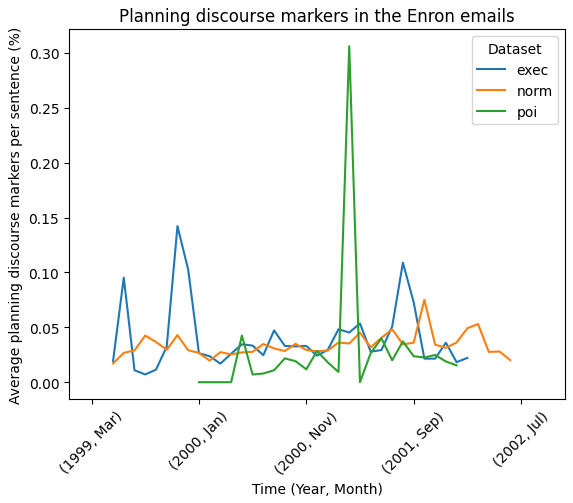
\includegraphics[width=8cm]{images/discourse_plot.png}
%         \caption{Need caption...}
%         \label{fig:discourse}
%     \end{subfigure}
%     \caption{Planning discourse markers in Enron emails}
%     \label{fig:politeness_discourse}
% \end{figure}


\begin{figure}[t]
    \centering
    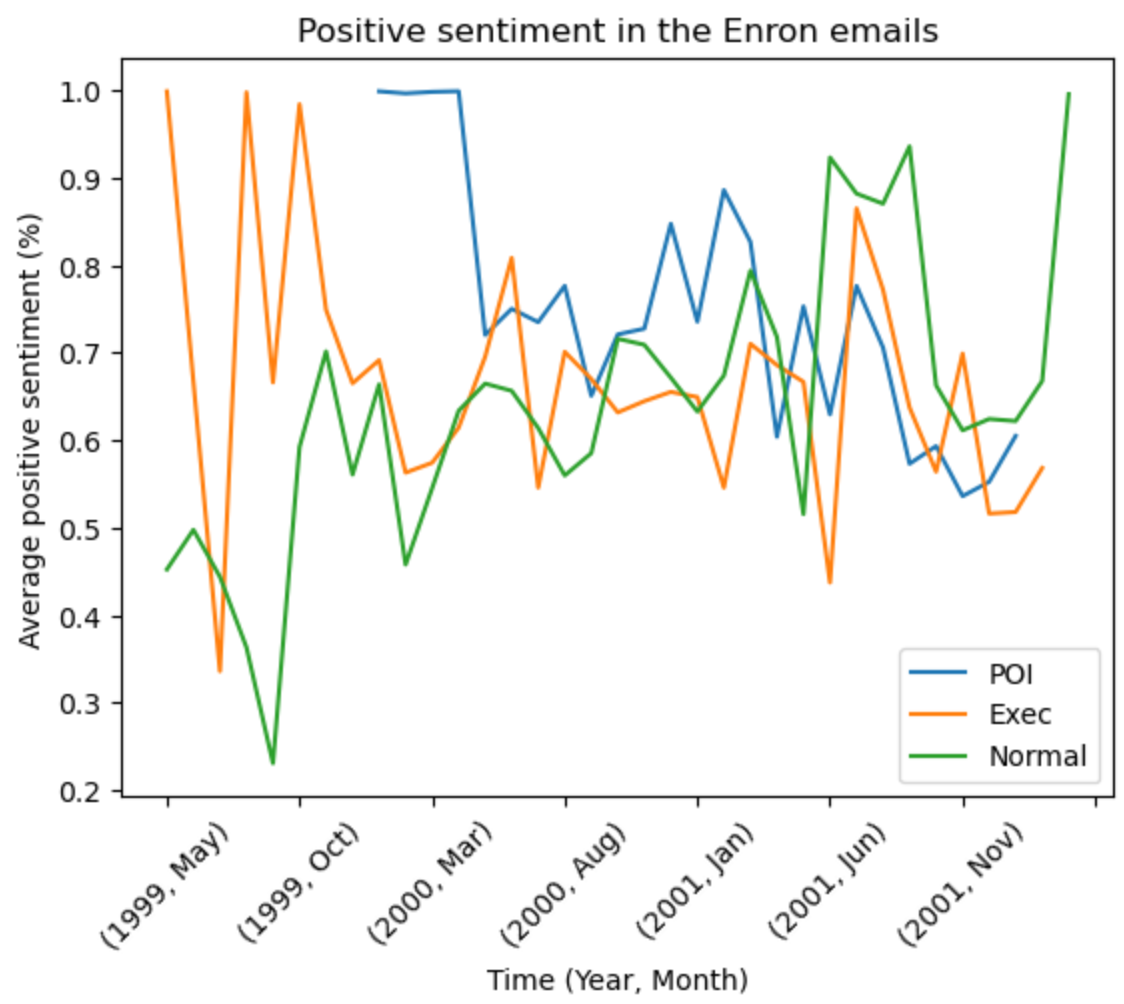
\includegraphics[width=8cm]{images/sentiment_plot.png}
    \caption{Sentiment fluctuation in Enron emails}
    \label{fig:sentiment}
\end{figure}

\begin{table}[b]
    \centering
    \begin{tabular}{|l|l|}
    \hline
    \textbf{Metric}            & \textbf{Value} \\ \hline
    Preprocessing               & Lemmatization + Unigram \\ \hline
    Model Class                & Logistic Regression (C=10) \\ \hline
    Precision         & 0.8204 \\ \hline
    Recall            & 0.8335 \\ \hline
    F1 Score          & 0.8170 \\ \hline
    Accuracy          & 0.8335 \\ \hline
    \end{tabular}
    \caption{Best Model Performance Metrics}
    \label{tab:best_model_metrics}
\end{table}

\begin{figure}[t!]
    \centering
    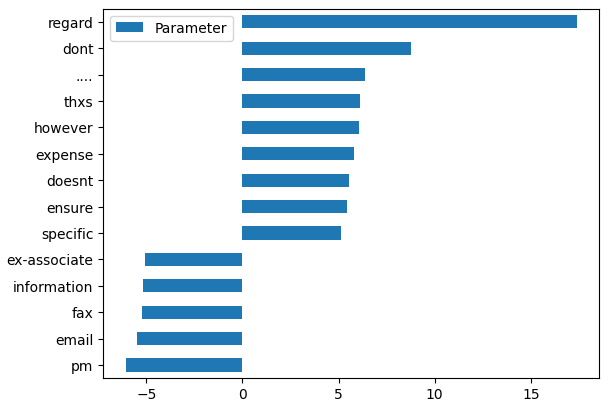
\includegraphics[width=8cm]{images/important_word_plot.png}
    \caption{Parameter weights for the top 14 features deemed most useful for detecting emails written by fraudulent/deceptive actors, as suggested by our best classifier}
    \label{fig:features}
\end{figure}



\section{Discussion and Conclusion}
% \textbf{What conclusions can be drawn from your experiments? Was your initial hypothesis verified? What are the limitations of your work, and how could it be extended?}

% Sentiment classifier (hugging face ref) to test the hypothesis that negative sentiment correlates with fraud... Not sure if this is relevant here... Will find place later.

Results in Figures \ref{fig:politeness} and \ref{fig:discourse} align well with the hypotheses in \cite{diplomacy}, namely that increased politeness and planning discourse markers are cues related to deception. This gives credence to the conjecture that these linguistic cues are indeed useful in more complex environments beyond games, and are general traits related to deceptive behaviour.

Most notably, it is interesting that planning discourse markers increase dramatically at the very beginning of the collapse and then subside, even as further events are unfolding, whereas politeness increases gradually up to the very collapse. This is an interesting addition to the results in \cite{diplomacy}. Diplomacy covers a short time span, whether measured by physical time or by number of events leading up to the deception. It is therefore not surprising that all deception markers overlap. In the case of Enron, the collapse was unfolding over a year, leaving more space between events, and therefore more time for deception markers to develop. %It would be interesting to look further into whether planning discourse markers regularly precede increased politeness in the course of deception. 

The fact that our results align with the ones in \cite{diplomacy}, though the alignment is not perfect, gives us some food for thought. %, as we labour in a very different setting altogether. 
In particular, since the emails analyzed are not directed at the targets of the deception (i.e., the shareholders and authorities), our findings suggest that an individual's general level of politeness increases when that individual engages in deception more generally. 

Furthermore, the results from our classifier training gives some interesting insights into the word usage of deceptive and non-deceptive actors. Most notable are the words with negative weights (therefore indicative of a non-POI email). There we observe words like ``fax" and ``email" which may be more associated with non-executive individuals. Additionally words like ``pm" suggest potential meetings which may be more commonplace for non-executive individuals.

These words may not be applicable to other settings, however additional work may be needed to confirm this.

\subsection{Limitations}

One major limitation of this work is that our classification of POIs only occurs based a single email, and does not account for prior context or email threads within its prediction. Doing so in such a situation could potentially give even more insightful cues in deception and potentially manipulation.
% Though our dataset contained over 13,000 emails, this may not be an appropriate size, and therefore represent appropriate difficulty, in detecting fraudulent actors in other settings. In this case, our approach was limited by the number of emails corresponding to the POIs, and more data could give better results.

% Aspects specific to the Enron dataset were also problematic. For example, almost all of the emails from Kenneth Lay's inbox were written by his assistant, which had to be discarded since they were not written by him. 
% This choice was made in order to preserve the linguistic qualities of the emails. However, it had several consequences, the obvious one being that we were left with very few emails from K. Lay, who was a major player in the Enron collapse, but also a top exec who rarely wrote his own emails. A message written by his assistant from his account was necessarily written at his behest. We have thus deprived ourselves of a large number of messages that would faithfully represent his intent. This is not a trivial loss, since deception is perpetrated both in content and in form (cite the italian papers or something ???) and we have restricted ourselves entirely to the form. 

Another limitation is that a large part of the deception at Enron was targeted at the general public. As such, interviews and public communications by POIs would have added valuable linguistic cues that are not included in our analysis. 

\subsection{Future work} 

% The discrepancy between the negative words identified as positive features for predicting POIs by our classifier, and our finding that negative sentiment is an area for more exploration. 
Incorporating models that can handle email context and email threads within their predictions would be an important step towards better understanding deception. 

Another interesting direction would be to test whether toxicity relates to fraud. This would be consistent with the results of our classifier and to some extent with \cite{hubris} seeing as toxicity and hubris can be linked.

% As mentioned above, another avenue for future work would be to investigate how the various deception markers are deployed relative to each other. Based on our meager evidence, we conjecture that an increase in planning discourse may be of shorter duration and may occur at the start of the deceptive practices, whereas politeness may increase throughout the deception. This also follows some common sense intuition. Given that planning discourse is more resource intensive and more deliberate, it makes sense that it be used parsimoniously and reluctantly. Politeness, on the other hand, can be thought of as a (conscious or subconscious) compensation technique, and therefore be used increasingly as the deception proceeds. 

\subsection{Conclusion}
We explored the possibility of identifying emails written by a fraudster based solely on their language using the Enron email dataset. We found that politness and planning discourse markers increased in frequency around the collapse, but sentiment did not appear related to deception. Our linear classifer acheieved good F1 score indicating that it is possible to identify POIs even among other executives. More research is required to validate the features identified by our models.

% In this paper we explore the possibility of identifying
% a fraudster based on their language. To this end, we consider the
% data set of emails of Enron employees, ranging from convicted
% offenders to regular employees. We look at fraud through the prism
% of deception, verifying if known markers of deception correlate
% with fraud. We also look for new potential language markers that
% could correlate to fraud.



\section{Statement of Contributions}

All team members contributed equally to the design of the project. D. Hobson and C. Moses processed the emails. S. Vassileva performed the sentiment analysis, D. Hobson tackled politeness and trained the classifiers and C. Moses analysed the discourse markers. All team members contributed to writing the report. 


%%%%%%%
%Everyone contributed to design of project.
%
%David and Caleb did email processing.
%
%Svetla did sentiment.
%David did politeness.
%Caleb did discourse markers.
%
%David trained classifiers.
%
%Everyone contributed to writing.

% Entries for the entire Anthology, followed by custom entries
\bibliography{references}
\bibliographystyle{acl_natbib}

% \appendix

% \section{Example Appendix}
% \label{sec:appendix}

% This is a section in the appendix.

\end{document}
